\section{Materiales y métodos} \label{seccion:MaterialesMetodos}

\subsection{Materiales}

En primer lugar, la \textbf{base de datos se puede obtener} del repositorio de \textit{Kaggle} \cite{database:online}.

Como ya se ha comentado previamente, la base de datos se compone de registros con métricas de candidatos en entrevistas de trabajo de pruebas (para entrenar a los candidatos en estas entrevistas), junto con si el candidato es escogido o no para el hipotético puesto de trabajo.

El conjunto de datos se compone originalmente de 10 columnas (variables) y 2983 filas (registros). Las variables que contiene la base de datos son las siguientes:

\begin{enumerate}
    \item Identificador numérico del estudiante. Lo llaman nombre del estudiante, pero en verdad se corresponde con una etiqueta numérica del tipo \entrecomillado{Student \textless id \textgreater}
    \item Apariencia general
    \item Formas de hablar
    \item Condición física
    \item Agilidad mental
    \item Confianza en si mismo
    \item Habilidad para presentar ideas
    \item Habilidades de comunicación
    \item Rendimiento académico
    \item Empleabilidad
\end{enumerate}

Todas las variables, salvo el identificador y la empleabilidad, son variables discretas tomando valores del 1 al 5. La estructura del identificador ya la hemos comentado. Y la empleabilidad toma dos valores de tipo \textit{string}: empleable o no empleable.

En \cite{database:online}, se comenta que la base de datos no ha sido tratada de ningún modo. Sin embargo, podemos inspeccionar la base de datos manualmente. El identificador llega hasta un valor de 3000, pero solo tenemos 2983 filas. Como vemos más adelante, no tenemos valores faltantes, así que asumimos con bastante seguridad que las 17 filas que faltan tenían valores faltantes, y se han borrado.

No usamos para nada el identificador del estudiante, así que de ahora en adelante, nos podemos olvidar de esa variable. Mostramos ahora algunos estadísticos básicos sobre el conjunto de datos sin tratar:

\begin{table}[H]
\scalebox{0.8}{
\begin{tabular}{lllllllll}
    Variable &  Mínimo & Máximo & 1º Cuartil  & Media & Mediana & 3º Cuartil & Desv. Típica \\
    \hline
    Agilidad mental & 2.0 & 5.0 & 3.0 & 3.963 & 4.0 & 5.0 & 0.7814509 \\
    Rendimiento académico & 3.0 & 5.0 & 4.0 & 4.611 & 5.0 & 5.0 & 0.6895586 \\
    Formas de hablar & 2.0 & 5.0 & 3.0 & 3.885 & 4.0 & 4.0 & 0.7527855 \\
    Condición física & 2.0  & 5.0  & 3.0  & 3.972  & 4.0  & 5.0 & 0.7466378 \\
    Apariencia & 2.0 & 5.0 & 4.0 & 4.247 & 4.0 & 5.0 & 0.6824864 \\
    Confianza & 2.0 & 5.0 & 3.0 & 3.911 & 4.0 & 5.0 & 0.8074833\\
    Habilidad para presentar ideas & 2.0 & 5.0 & 3.0 & 3.814 & 4.0 & 4.0 & 0.7339429 \\
    Habilidades comunicativas & 2.0 & 5.0 & 3.0 & 3.525 & 3.0 & 4.0 & 0.7371541 \\

\end{tabular}
}
\caption{Resumen del conjunto de datos original}
\end{table}

Con esto vemos que aunque las métricas van, en un diseño inicial, del valor 1 al 5, muchas de ellas tienen un rango más acotado (por debajo), puesto que no hubo participantes que obtuviesen los valores mínimos.

Al estar trabajando con variables discretas, el siguiente gráfico es muy útil a la hora de visualizar la distribución de los datos:

\begin{figure}[H]
    \centering
    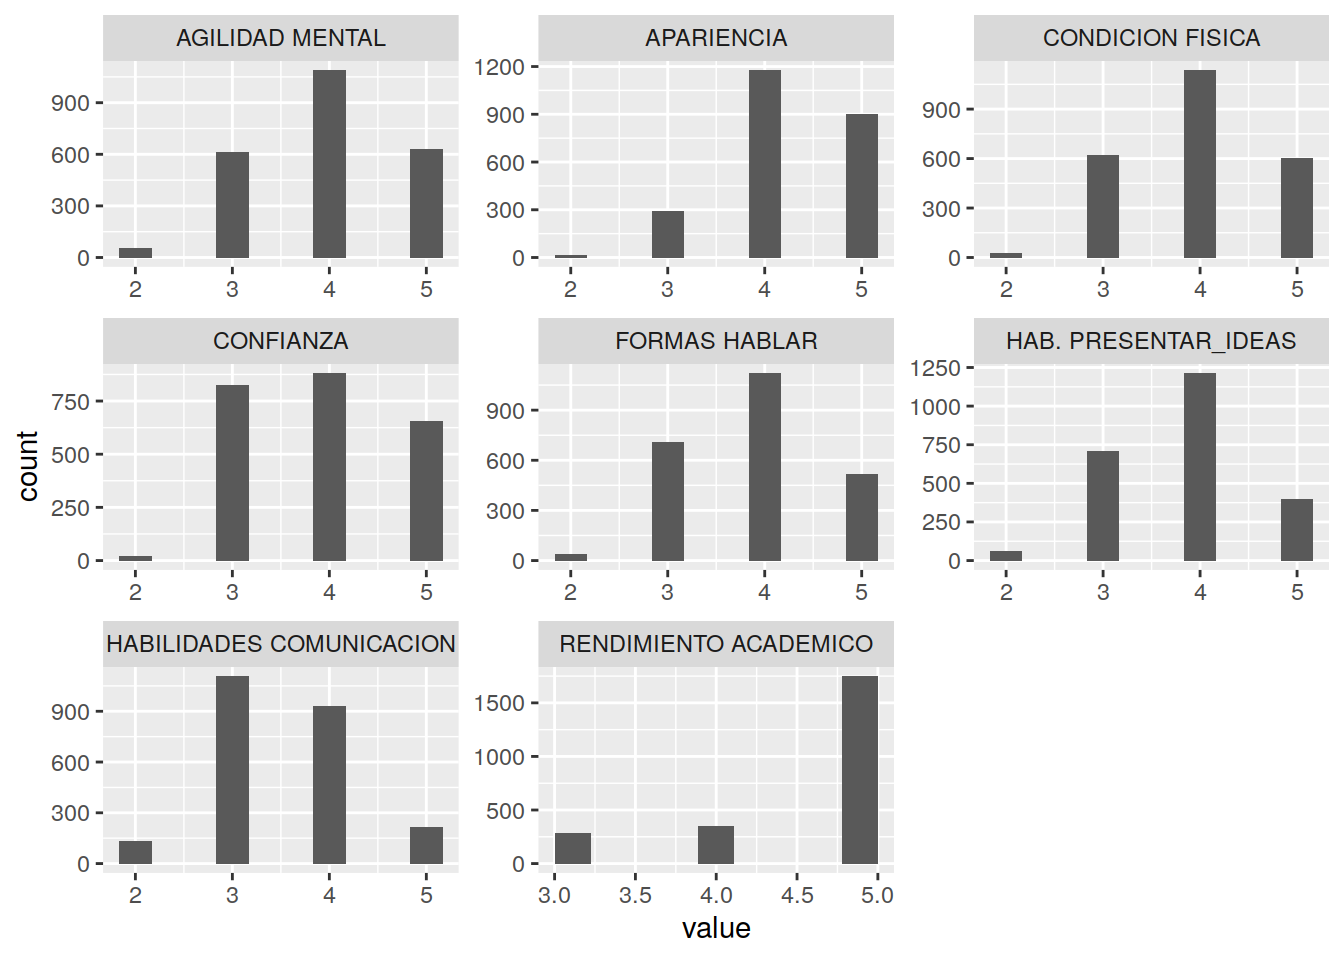
\includegraphics[width=0.8\textwidth]{histogramas_variables}
    \caption{Histograma de las variables de entrada}
    \label{fig:histogramas_variables}
\end{figure}

Mostramos gráficamente la distribución de la variable de salida:

\begin{figure}[H]
    \centering
    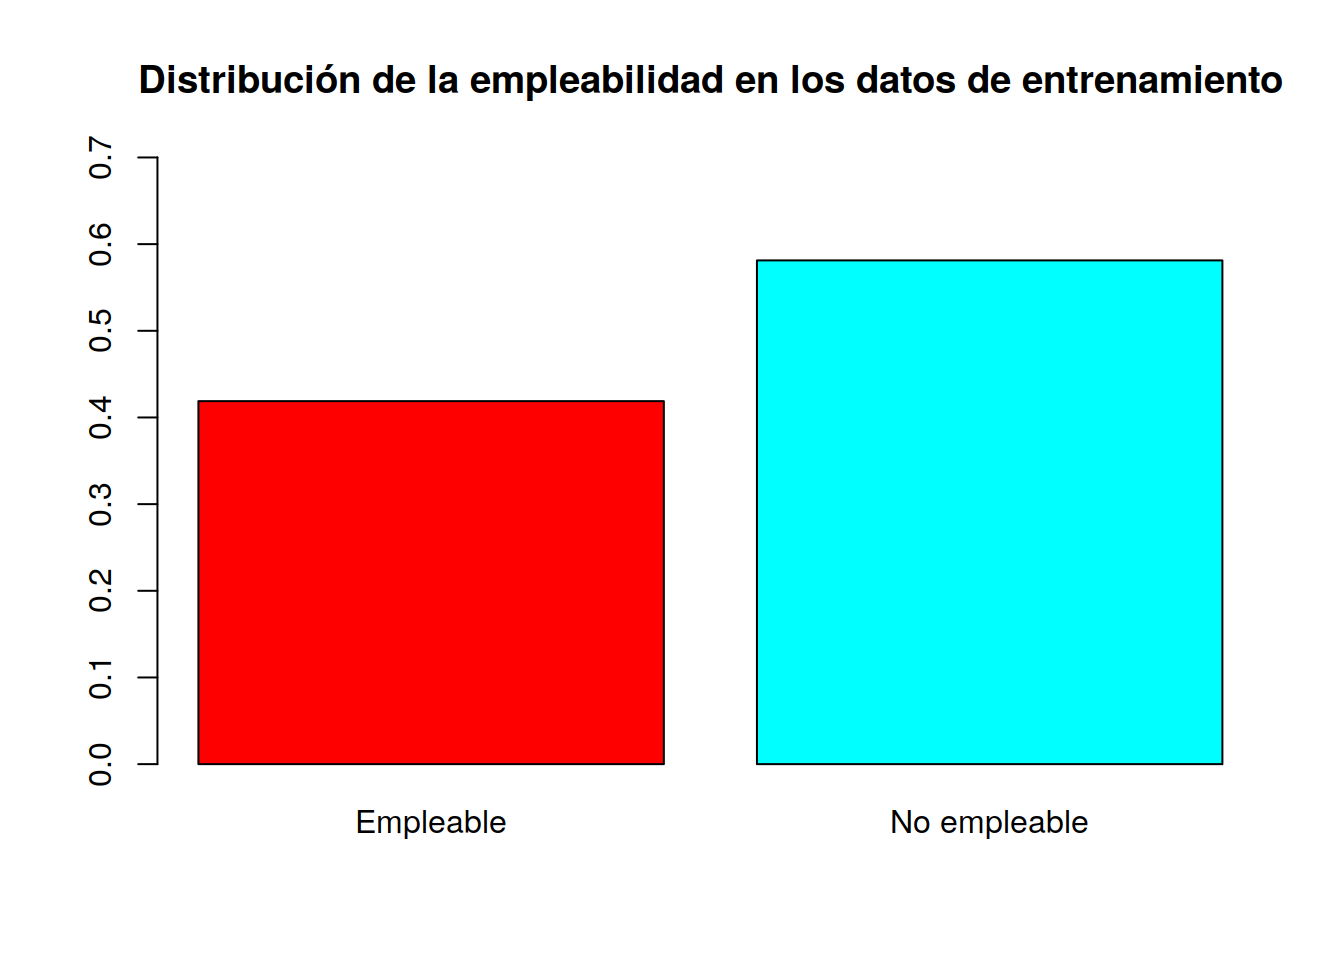
\includegraphics[width=0.6\textwidth]{balanceo_clases}
    \caption{Distribución de la variable de salida, con la que podemos estudiar el balanceo de las clases}
    \label{fig:balanceo_clases}
\end{figure}


Hay cierto desbalanceo hacia la no empleabilidad, aproximadamente un $40-60\%$. En general, este desbalanceo no es demasiado grave. Además, considerando el desbalanceo esperable dado el contexto en el que estamos (un porcentaje mayoritario no debería ser aceptado para un trabajo), consideramos que no necesitamos aplicar alguna técnica para tratar este desbalanceo (i.e. podría aplicarse \textit{SMOTE}).

\subsection{Métodos estadísticos}

Para el \textbf{análisis univariante}, usamos los siguientes métodos:

\begin{itemize}
    \item Separación en entrenamiento y \textit{test} para una futura validación cruzada (80\% - 20\%)
    \item Recodificación del \textit{string} de la variable de salida, en valores $0, 1$ y con un \textit{factor} de \textit{R}
    \item Gráficos de cajas
    \item Análisis univariante de \textit{outliers}, usando rangos intercuartílicos
    \item Test de normalidad univariante: test de \textit{Shapiro-Wilk}
\end{itemize}

Para el \textbf{análisis multivariante}, usamos:


\begin{itemize}
    \item Matriz de correlaciones, test de correlación: test de esfericidad de \textit{Bartlett}
    \item Análisis multivariante de \textit{outliers} usando la distancia de \textit{Mahalanobis}
    \item Estandarización de las variables
    \item Componentes Principales. Para elegir el número de componentes principales:
        \begin{itemize}
            \item Regla de \textit{Abdi}
            \item Mínimo de Varianza explicada
            \item Método del codo
            \item Análisis paralelo
        \end{itemize}
    \item Análisis Factorial. Para elegir el número de variables latentes:
        \begin{itemize}
            \item Método del codo
            \item Análisis paralelo
        \end{itemize}
    \item Test de normalidad multivariante: test de \textit{Mardia} y test de \textit{Henze-Zirkler}
    \item Test de la homogeneidad de la varianza: test \textit{Box M}
\end{itemize}

Para la \textbf{exploración de los hiperparámetros}, necesarios para la futura clasificación, usamos \footnotemark:

\footnotetext{Tenemos tres conjuntos de datos con los que podemos construir un clasificador. También estamos trabajando con tres modelos distintos. Así que realizamos esta exploración de hiperparámetros para escoger entre las nueve combinaciones posibles.}

\begin{itemize}
    \item Los tres modelos clasificadores: discriminante lineal, discriminante cuadrático y \textit{XGBOOST}
    \item \textit{k-Fold Cross Validation} como método estadístico para realizar la búsqueda de hiperparámetros. Usamos 10 \textit{folds}.
\end{itemize}

Para la \textbf{clasificación}, aunque escogemos la mejor combinación de modelo-conjunto de datos, entrenamos sobre los tres modelos, en cada uno usando el mejor conjunto de datos para ese modelo.

Además, estudiamos las importancias de las variables a la hora de construir el modelo (en \textit{LDA} y \textit{XGBOOST}).

Para la \textbf{validación de los modelos}, usamos:

\begin{itemize}
    \item \textit{Accuracy} sobre entrenamiento y \textit{test}
    \item Matriz de confusión
\end{itemize}

Y para finalizar, en el \textbf{experimento adicional}, usamos:

\begin{itemize}
    \item Separación de la base de datos en función de si tenemos variables meritocráticas o no
    \item Ajuste de hiperparámetros de \textit{XGBOOST} usando \textit{k-Fold Cross Validation} y \textit{Grid Search}
    \item Validación de los resultados obtenidos con el \textit{accuracy} y matriz de confusión
\end{itemize}


